\documentclass[10pt,a4paper,english]{article}
\usepackage{geometry,metalogo,hyperref,babel,mdwlist,multicol,parskip}
\usepackage[default]{comicneue}
\usepackage[scaled=.9]{sourcecodepro}

\hypersetup{colorlinks,citecolor=blue,filecolor=blue,linkcolor=blue,urlcolor=blue}
\NewDocumentCommand\file{m}{\href{run:#1.pdf}{#1}}
\NewDocumentCommand\cmd{m}{\texttt{\bfseries \textbackslash #1}}

\title{%
	\vspace{-4em}
	\comicneuelight
	\resizebox{\linewidth}{!}{comicneue}\\
	\resizebox{\linewidth}{!}{Craig Rozynski's Comic Neue fonts for \LaTeX}
}

\author{Silke Hofstra, \href{mailto:tex@slxh.nl}{tex@slxh.nl}}
\date{Documentation for comicneue v1.0.\\ \today}
\listfiles
\begin{document}
\maketitle
\begin{multicols}{2}
This package provides the Comic Neue fonts in an easy to use way.
For \XeLaTeX\ and \LuaLaTeX\ users the original OpenType fonts are used.
The entire font family is included.

Comic Neue is a redesign of the infamous Comic Sans font.
More information about this redesign can be found on \href{http://comicneue.com/}{comicneue.com}.

This package is also available on \href{https://github.com/silkeh/latex-comicneue}{GitHub}.

\section{Options}
The package has the following options:
\begin{itemize*}
	\item \textbf{light}:          use the light weight by default.
	\item \textbf{regular}:        use the regular weight by default.
	\item \textbf{angular}:        Use the angular variant instead of the normal one.
	\item \textbf{scale}:          Change the scaling with a factor. For example:  \texttt{scale=.5}
	\item \textbf{default}:        Sans-serif is set as default font family.
	\item \textbf{sfdefault}:      Comic Neue is set as sans-serif family.
	\item \textbf{nosfdefault}:    Comic Neue is not set as sans-serif family.
	\item \textbf{type1, t1}:      Override automatic detection and use the Type 1 fonts.
	\item \textbf{opentype, otf}:  Override automatic detection and use OpenType fonts.
\end{itemize*}
The following options are enabled by default: sfdefault, regular.

\section{Commands}
Commands for all weights and styles are also provided:
\begin{itemize*}
	\item \cmd{comicneue}
		-- the regular and bold weights.
	\item \cmd{comicneuelight}
		-- the light and bold weights.
	\item \cmd{comicneueangular}
		-- the regular and bold weights in the angular style.
	\item \cmd{comicneuelight}
		-- the light and bold weights in the angular style.
\end{itemize*}

\section{Licence}
The Comic Neue fonts are available under the \href{http://scripts.sil.org/OFL}{SIL Open Font License}.\\
All \LaTeX\ code is available under the \href{http://www.latex-project.org/lppl/}{\LaTeX\ project public license} v1.3 or later.

\section{Specimen}
Simple specimen are included on page \pageref{sec:specimen}.

\section{Version history}

\subsection*{1.0}
\begin{itemize*}
	\item Initial release with v2.2 of the fonts.
\end{itemize*}

\end{multicols}

\clearpage

\section{Specimen}
\label{sec:specimen}
\subsection{OpenType}
\begin{figure}[ht]
	\centering
	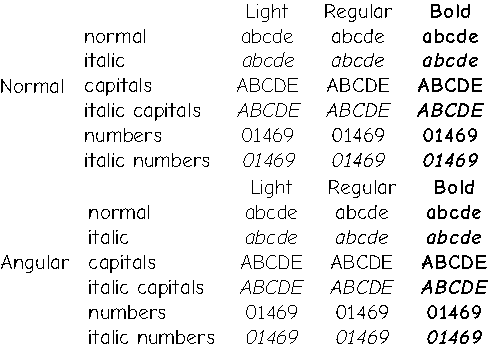
\includegraphics[width=.7\textwidth]{comicneue-otf-specimen}
\end{figure}
This table can also be found in \file{comicneue-otf-specimen}.

\subsection{Type1}
\begin{figure}[ht]
	\centering
	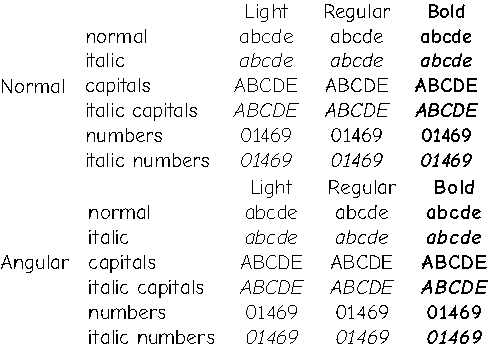
\includegraphics[width=.7\textwidth]{comicneue-type1-specimen}
\end{figure}
This table can also be found in \file{comicneue-type1-specimen}.

\end{document}

